% Author Vahid Partovi Nia
% Copyright Huawei Technologies
% Network Mind Team



\documentclass[12pt]{beamer}

\usetheme{Hannover}
\setbeamercolor{section in sidebar shaded}{fg=black}

\usecolortheme{beaver}
\beamertemplatenavigationsymbolsempty

%  \usebeamertemplate{navigation symbols}\hfill
%  \insertframenumber{}/\inserttotalframenumber}
  

\useoutertheme{sidebar}
\pgfdeclareimage[width=2.5\baselineskip]{institut-logo}{fig/mcgill_logo}
\setbeamertemplate{footline}
{\raisebox{-2ex}{\pgfuseimage{institut-logo}}
%  \hfill
\hspace{5cm}
  \usebeamertemplate{navigation symbols}
  \insertframenumber{}/\inserttotalframenumber
  \hspace{3.8cm}
YCBS255
}
%\setbeamertemplate{sidebar right}{}
  
\setbeamercolor{block title}{fg=darkred}
\setbeamercolor{local structure}{fg=darkred}

\setbeamercolor{palette sidebar secondary}{fg=darkgray, bg=white}



\usefonttheme{professionalfonts} % using non standard fonts for beamer


\makeatletter
\beamer@nav@subsectionstyle{hide/hide/hide}
\makeatother

\titlegraphic{
\includegraphics[width=2cm]{fig/mcgill_logo}}




\usepackage{listings}

\def \y {\mathbf y}
\def \X {\mathbf X}
\def \A {\mathbf A}
\def \t {^\top}
\def \inv {^ {-1}}
\def \x {\mathbf x}
\def \bbeta {\boldsymbol \beta}
\def \eeps {\boldsymbol \varepsilon}
\def \TV {\mathrm{TV}}
\def \Radio {\mathrm{Radio}}
\def \Newspaper {\mathrm{Newspaper}}
\def \Sales {\mathrm{Sales}}


\begin{document}

% no title and no author on sidebar
\title[]{Linear Regression}   
\author[]{Vahid Partovi Nia} 
\institute{Lecture 02: Simple and Multiple Linear Regression}
\date{30 October 2018}


\makeatletter
  \begin{frame}[plain]
    \hspace*{-\beamer@leftsidebar}%
    \advance\textwidth by \beamer@leftsidebar\relax
    \beamer@leftsidebar=\z@
    \begin{minipage}{\textwidth}\par%
      \maketitle
    \end{minipage}
  \end{frame}
  \makeatother



\frame{\frametitle{Outline}\tableofcontents} 

\setbeamertemplate{sidebar left}[sidebar theme]


\section{Terminology}


\frame{\frametitle{Equivalent terminologies}
\begin{itemize}
\item $y$: dependent variable, response variable, output variable 
\item $x$: independent variable, explanatory variable, input variable, feature. 
\end{itemize}
}


\frame{\frametitle{Supervised Learning}
\begin{itemize}
\item Regression: $y$ is continuous
\item Classification: $y$ is discrete
\end{itemize}
}



\frame{\frametitle{Sales prediction}
$$y_1= 22,\quad y_2 = 10, \quad y_3 = 9,\quad y_4 = 18$$
$$y_i = \beta_0 + \varepsilon_i$$
\begin{itemize}
\item What is $\hat y_i$?
\item What is $\hat \beta_0$? 
\item Least squares: $ \min{{1\over 5}  \{(22-\beta_0)^2 + \cdots+(18-\beta_0)^2}$
\item $\hat \beta_0 = {1\over 5} (22 + \cdots + 18)$
\end{itemize}
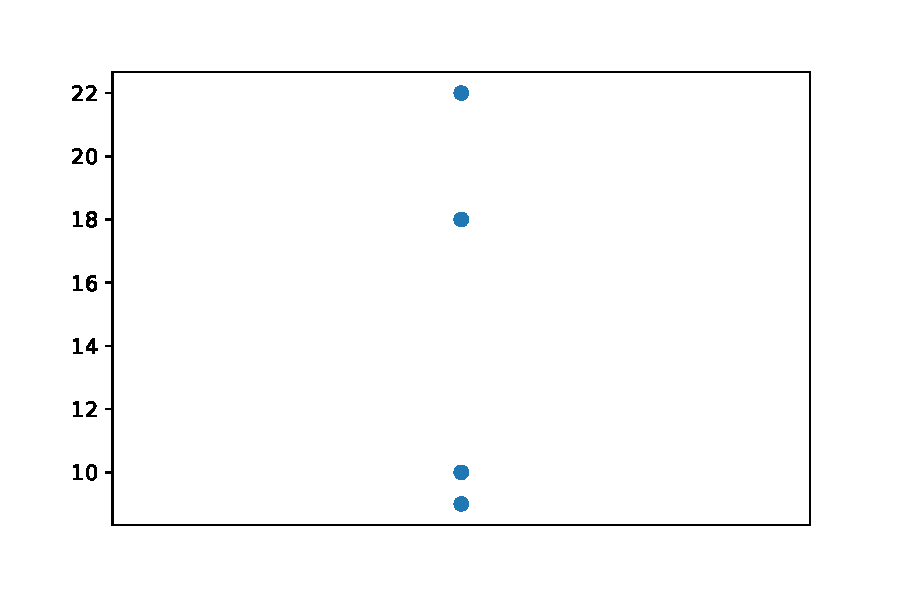
\includegraphics[width=0.4\textwidth]{fig/sales}\\
}


\section{Advertisement}


\frame{\frametitle{Advertisement}
Suppose we have a fixed budget of advertisement to increase sales. 
\begin{block}{Problem:} 
How do you distribute advertisement budget between different advertisement methods? 
\end{block}

\pause
TV, Radio, Newspaper, Online, etc.
\begin{exampleblock}{Question:} 
\begin{itemize}
\item Does advertisement affect sale? 
\item How do we predict sale?
 \item What is $y$ what is $x$?
 \item Is it a regression or a classification? 
\end{itemize}
\end{exampleblock}
}

\frame{\frametitle{sales vs ad}
$\textrm{Sales:~} y $\\
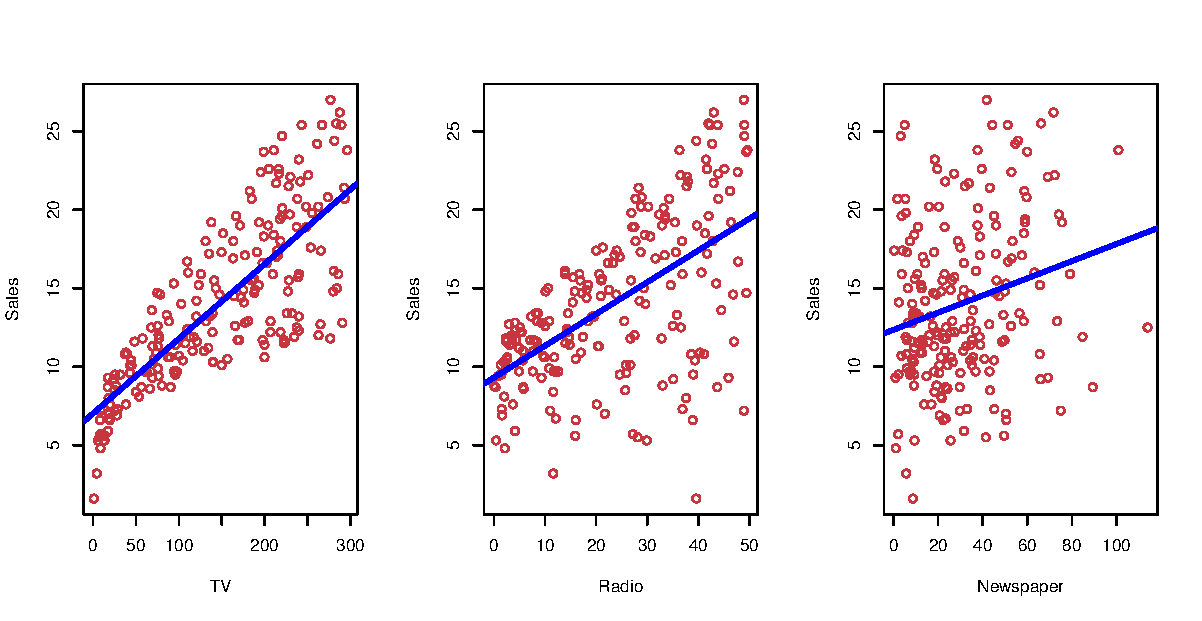
\includegraphics[width=\textwidth]{fig/2-1}\\
$\quad  \quad \textrm{TV:~} x_1  \quad\quad \quad \quad\quad \textrm{Radio:~} x_2 \quad \quad \quad \textrm{Newspaper:~ } x_3$
\begin{eqnarray*}
\textrm{Learning:~} \Sales &\approx& f(\TV, \Radio,\Newspaper)+\varepsilon\\
\end{eqnarray*}
}

\frame{\frametitle{Sale prediction simplification}
\begin{eqnarray*}
\Sales &\approx& f(\TV,\Radio,\Newspaper)\\
&\Downarrow&\\
 \Sales &\approx& f_1(\TV) + f_2(\Radio) + f_3(\Newspaper)\\
&\Downarrow&\\
\Sales&\approx& f_1(\TV)\\
&\Downarrow&\\
y &\approx& \beta_0 +\beta_1 \TV \\
&\Downarrow&\\
y &\approx& \beta_0 \\
\end{eqnarray*}
}

\frame{\frametitle{Python}
Step 1
\begin{itemize}
\item Load ``Advertising.csv"
\begin{itemize}
\item path='/Users/Desktop/datafiles/'
\item filename=path+'Advertising.csv' 
\end{itemize}
\item \texttt{import pandas as pd}
\item \texttt{import numpy as np}
\item Take the mean of  ``sales"
\end{itemize}
}


\begin{frame}[fragile]
\tiny
\begin{lstlisting}
import pandas as pd
path='data/'
filename = path+'Advertising.csv'
advertising = pd.read_csv(filename)
\end{lstlisting}
\begin{lstlisting}
import numpy as np
np.mean(advertising['sales'])
\end{lstlisting}
\end{frame}


\frame{\frametitle{Simple linear regression}
\begin{tabular}{c c c c}
$y_1= 22$         & $y_2 = 10$   & $y_3 = 9$      & $y_4 = 18$ \\
$x_{11} = 230$ & $x_{12}= 44$ & $x_{13}=17$ & $x_{14}= 151$
\end{tabular}
\begin{center}
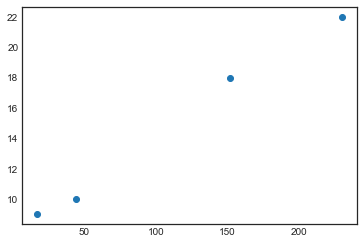
\includegraphics[width=0.4\textwidth]{fig/salestv}
\end{center}
$$y_i = \beta_0 + \beta_1 x_{1i}+\varepsilon_i$$
What is $\hat y_i$?
}

\section{Simple Linear Regression}

\frame{\frametitle{Simple linear regression}
Step 2: Predict $\Sales$ using $\TV$
\begin{itemize}
\item Load ``LinearRegression" from sklearn\
\item Initialize the model
\item Feed the data
\item Scatter plot $\Sales$ versus $\TV$ 
\item Add the predicted line
\end{itemize}
}


\begin{frame}[fragile]
\tiny
\begin{lstlisting}
from sklearn.linear_model import LinearRegression
lr = LinearRegression()
\end{lstlisting}
\pause
\begin{lstlisting}
lr.fit(X = advertising[ ['TV'] ], y = advertising['sales'])
print(lr.intercept_, lr.coef_)
\end{lstlisting}
\pause
\begin{lstlisting}
import matplotlib.pyplot as plt
%matplotlib inline
\end{lstlisting}

\begin{lstlisting}
plt.plot(advertising.TV, advertising.sales, 'or', mfc='none');
plt.plot(advertising.TV, lr.intercept_+lr.coef_*advertising.TV, '-b');
\end{lstlisting}

\begin{lstlisting}
plt.xlabel('TV');
plt.ylabel('sales');
\end{lstlisting}

\end{frame}


\section{Multiple Linear Regression}

\frame{\frametitle{Combine models}
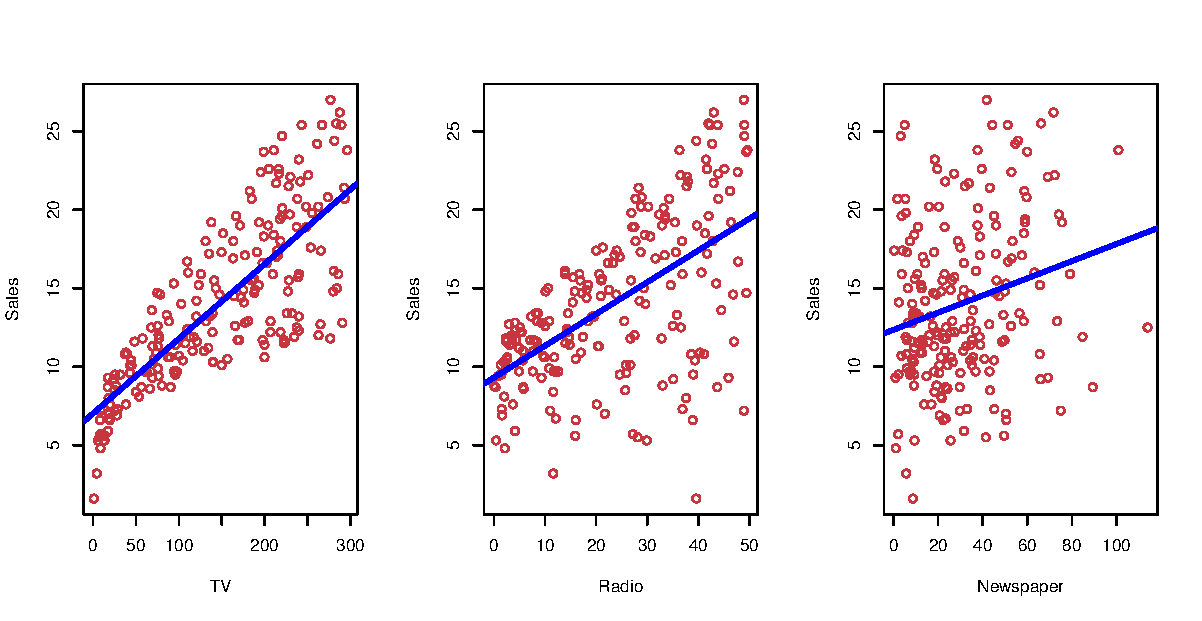
\includegraphics[width=\textwidth]{fig/2-1}\\
$\quad  \quad \textrm{TV:~} x_1  \quad\quad \quad \quad\quad \textrm{Radio:~} x_2 \quad \quad \quad \textrm{Newspaper:~ } x_3$
\begin{eqnarray*}
\Sales &=& \beta_0 + \beta_1 \TV + \beta_2 \Radio + \beta_3 \Newspaper+\varepsilon\\ 
\end{eqnarray*}
\pause 
Predict for $\TV = 250, \Radio = 30, \Newspaper = 20$
}


\begin{frame}[fragile]
\tiny
\begin{lstlisting}
lr = LinearRegression()
\end{lstlisting}
\pause
\begin{lstlisting}
lr.fit(X = advertising[ ['TV', 'radio', 'newspaper'] ], 
       y = advertising['sales'])

x = np.array([250, 30, 20] )
lr.predict(x.reshape(1,3))
\end{lstlisting}
\pause
\begin{lstlisting}
x = np.array([250, 30, 20, 249, 29, 19] )
lr.predict(x.reshape(2,3))
\end{lstlisting}
\end{frame}

\begin{frame}[fragile]
\tiny
\begin{lstlisting}
import statsmodels.formula.api as smf
model = smf.ols(formula='sales ~ TV + radio + newspaper', 
		data = advertising)
lr = model.fit()
lr.summary()
\end{lstlisting}
\end{frame}

\frame{\frametitle{ols summary}
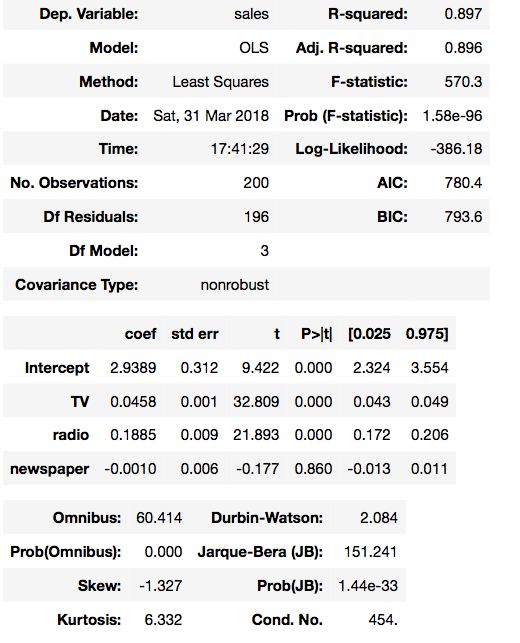
\includegraphics[width=0.5\textwidth]{fig/olsall}
}

\section{Education}


\frame{
$\textrm{Income:~} y $ \\
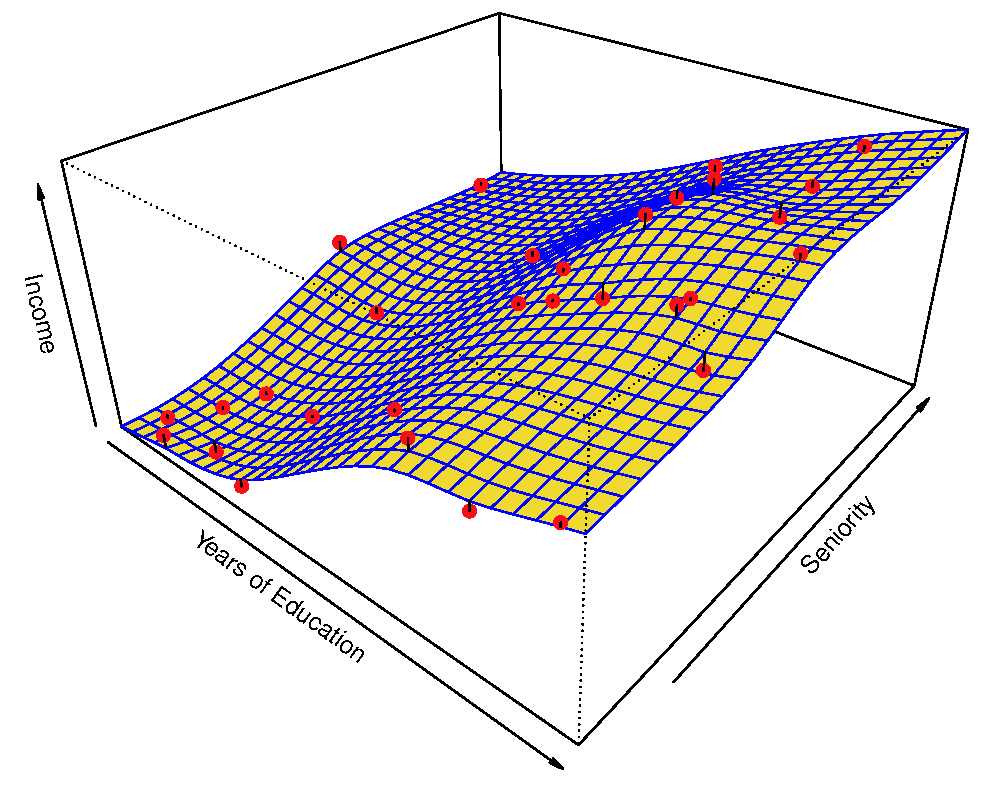
\includegraphics[width=0.8\textwidth]{fig/2-5}\\
$ \textrm{Years of Education:~} x_1\quad\quad \textrm{Seniority:~}   x_2 $\\
$y\approx f(x_1, x_2)$
}


\frame{
$\textrm{Income:~} y $ \\
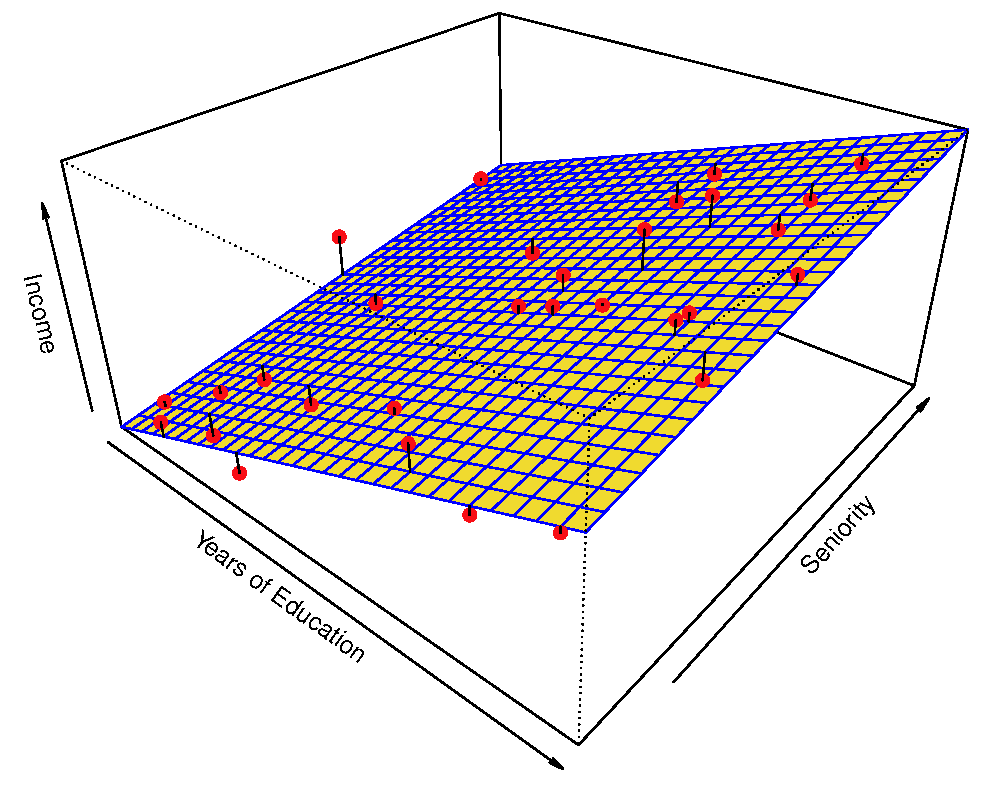
\includegraphics[width=0.8\textwidth]{fig/2-4}\\

\begin{eqnarray*}
y& \approx & \textcolor{blue}{f_1(x_1)} + \textcolor{green}{f_2(x_2)}\\
y &\approx& \beta_0+   \textcolor{blue}{ \beta_1 x_1}+\textcolor{green}{\beta_2 x_2}\\
\end{eqnarray*}
}

%\section{Linear Regression}
%
%\frame{\frametitle{Notation $n$ observation, $p$ features}
%$\eeps = 
%\begin{pmatrix} \varepsilon_1 \\ \vdots \\ \varepsilon_n  \end{pmatrix}, 
%\y = \begin{pmatrix} y_1 \\ \vdots \\ y_n  \end{pmatrix}, 
%\x = \begin{pmatrix} x_1\\ \vdots \\ x_p  \end{pmatrix}, 
%\bbeta = \begin{pmatrix}  \beta_0 \\ \beta_1 \\ \vdots \\ \beta_p \end{pmatrix}$
%
%$$\X_{n\times p} = \begin{pmatrix} \x_1\t \\ \vdots \\ \x_n\t \end{pmatrix} = \begin{pmatrix} 
%x_{11} & x_{12}&  \ldots & x_{1p} \\
%x_{21} & x_{22}&  \ldots & x_{2p} \\
%\vdots & \vdots&  \ddots & \vdots \\
%x_{n1} & x_{n2}&  \ldots & x_{np} \\
% \end{pmatrix}$$\\
% 
% $$\X_{n \times (p+1)}=
% \begin{pmatrix} 
%1 & x_{11}&  \ldots & x_{1p} \\
%1 & x_{21}&  \ldots & x_{2p} \\
%\vdots & \vdots&  \ddots & \vdots \\
%1 & x_{n1}&  \ldots & x_{np} \\
% \end{pmatrix}
% $$
%}
%
%
%\frame{\frametitle{Matrix differentiation}
%\begin{eqnarray*}
%\y &=& \X\bbeta +\eeps \\
%S(\bbeta) &=& (\y-\X\bbeta)\t (\y-\X\bbeta) 
%\end{eqnarray*}
%What is the minimizer of $S(\bbeta)$?
%\pause
%\begin{eqnarray*}
%{\partial \x \t \bbeta \over \partial \bbeta   } &=&  \x  \Rightarrow {\partial \X \bbeta \over \partial \bbeta   } =  \\
%{\partial \bbeta \t \A \bbeta \over \partial \bbeta   } &=& (\A + \A\t )\bbeta
%\end{eqnarray*}
%$ \hat \bbeta = (\X\t\X)\inv \X\t \y$\\
%How do we compute $\hat \bbeta$?
%}
%
%
%
%\frame{\frametitle{Numerical Consideration}
%\begin{itemize}
%\item Cholesky   is faster than LU 
%\item  LU is faster than QR 
%\item QR is faster than SVD \end{itemize} 
%}
%
%%
%%\frame{\frametitle{Numerical Questions}
%%\begin{itemize}
%%\item Why condition number of $(\X\t \X)$ is important?
%%\item What if the smallest eigenvalue of $\X\t \X$, say  $\lambda_p \approx 0$?
%%\item When does this happen in polynomial regression?
%%\item How to find LS if the polynomial order $k <n$?
%%\item How to find LS if the polynomial order $k \geq n$ ?
%%\end{itemize}
%%}
%%
%%
%%\section{Overfitting}
%%
%%\frame{\frametitle{Model Quality}
%%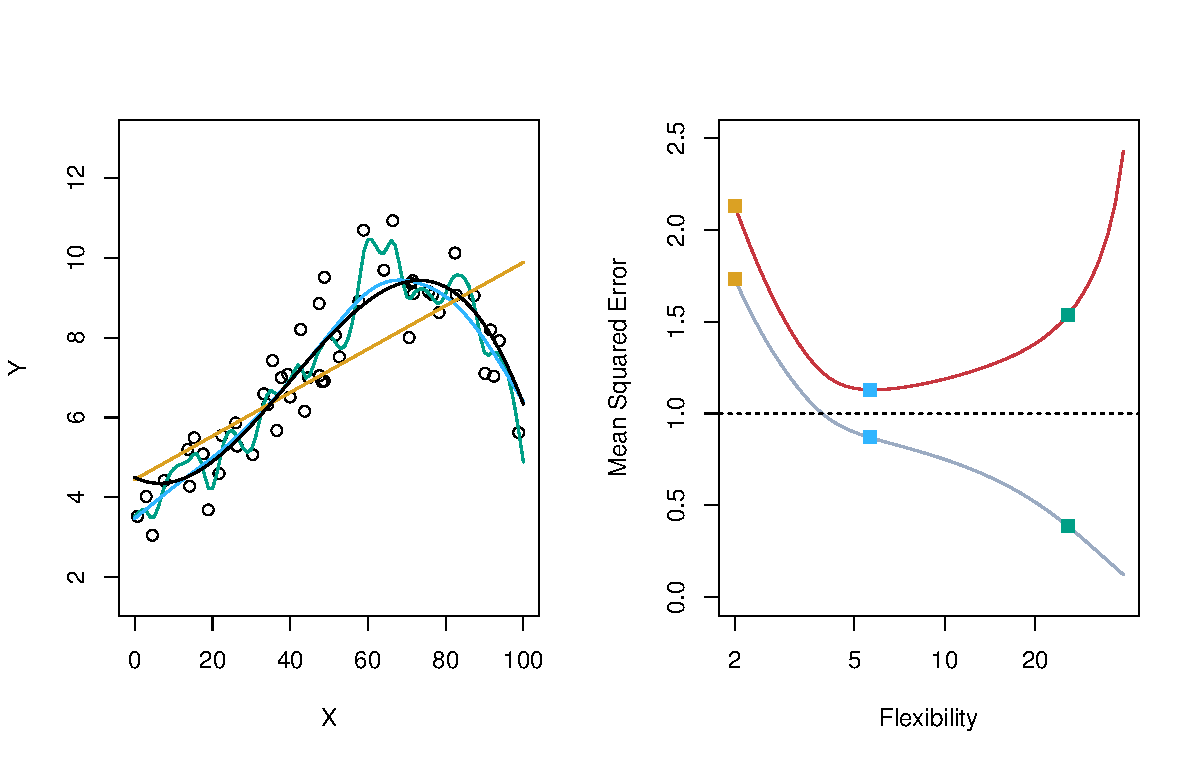
\includegraphics[width=0.9\textwidth]{fig/2-9}\\
%%Python code
%%}
%%
%
%
%%\frame{\frametitle{}
%%}
%
%%\frame{\frametitle{}
%%}
%
%
%
%

\end{document}
